
\begin{figure*}[h]
    \centering
    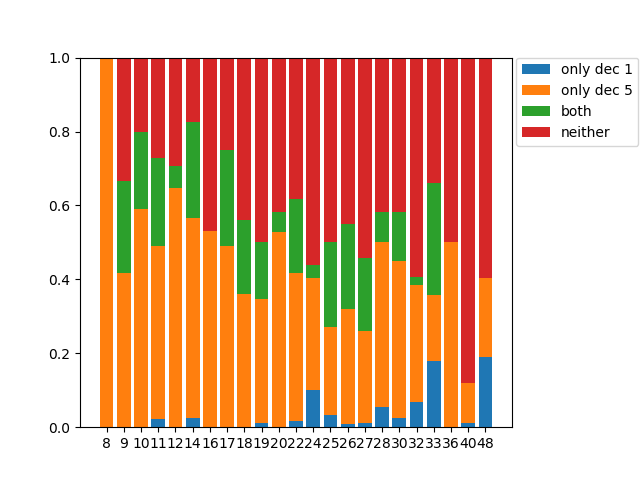
\includegraphics[width=.4\textwidth,keepaspectratio]{figures/jump_subset_out.png}
    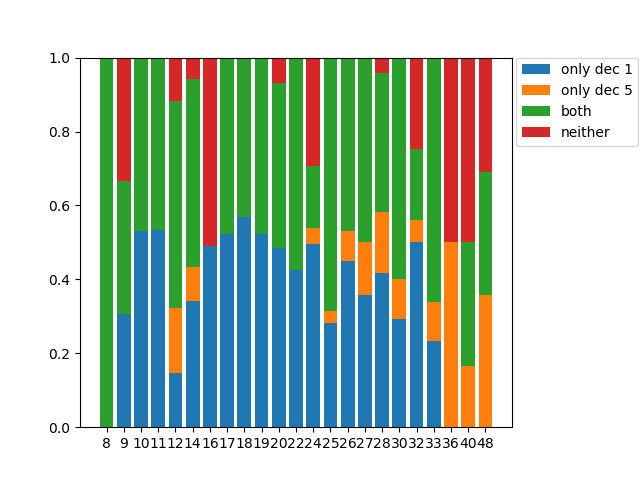
\includegraphics[width=.4\textwidth,keepaspectratio]{figures/template_subset_out.png}
    \caption{Performance distribution for jump and template splits with 5- and 1-decoder widths.}
    \label{fig:kernel_width}
\end{figure*}


\ldots For the random split, we observe the expected pattern in which
both wider encoder and decoder windows lead to better performance. The
jump results are less clear-cut, but respect the same trend: the
narrowest encoder-decoder combination shows the worst performance, and
the widest kernles combination the top one. For the around-right
split, it's also better to have the widest encoder, but now we find
that top performance is achieved with the \emph{narrowest} decoder
(width$=$1). Since the novel output templates in this split are by
construction long (as they involve executing an ``around'' command),
we would have rather expected models keeping track of a larger
decoding window to fare better. To gain some insight on the attested
behaviour, we looked at the performance distribution by output length
in the two splits. Keeping encoder width fixed at 5,
Fig.~\ref{fig:kernel_width} reports the proportions of cases that were
correctly handled only with decoder width 1, 5, both or neither, for
each ground-truth length. We plot statistics for the intersection of
the two generalization sets, but the same pattern is confirmed when
looking at the whole sets. We see more cases where both widths worked
in the around-right split, as expected, as we have already established
this as an easier challenge for our CNNs. In general, though, we find
that the wide-decoder jump model behaves quite similarly to the
narrow-decoder around-right model, getting most of its gains from
shorter sequences. One interesting difference is that, for
around-right, we observe an inversion in performance for the longer
sequences, where the wider decoder outperforms the narrower one, in
accordance with our intuition that more context should help longer
execution tasks. Looking qualitatively at the errors, we note that,
for both splits, the narrower decoder tends to skip trajectory
sub-chunks (e.g., executing ``jump around right'' with 3 instead of 4
right turns followed by jumps), whereas the wider kernel is more
likely to substitute actions (e.g., turning left instead of right) than
undershooting the length. Quantitatively, this is supported by the
fact that, for both splits, the narrow kernel errors have considerably
larger variance with respect to ground-truth length. While these
observations confirm the fact that a wider decoder kernel helps
with length management, we still have no insight on why the shorter
kernel should be better on the around-right split. Future work should
pursue a better understanding of how kernel widths affect linguistic
processing in CNNs.

